%%%% ijcai17.tex

\typeout{IJCAI-17 Instructions for Authors}

% These are the instructions for authors for IJCAI-17.
% They are the same as the ones for IJCAI-11 with superficical wording
%   changes only.

\documentclass{article}
% The file ijcai17.sty is the style file for IJCAI-17 (same as ijcai07.sty).
\usepackage{ijcai17}

% Use the postscript times font!
\usepackage{times}
\usepackage{booktabs} % For formal tables
\usepackage{verbatim}
\usepackage{fancynum}
\usepackage{graphicx}
\usepackage{bm}
\usepackage{amssymb}
\usepackage{tikz}
%\usetikzlibrary{bayesnet}
\usepackage{diagbox}
\usepackage{latexsym}
\usepackage{graphicx}
\usepackage{graphics}
\usepackage{amsmath}
\usepackage{natbib}
\usepackage{amsthm}       %% The amsthm package provides extended theorem environments
\usepackage{multirow}
\usepackage{algorithmic}
\newcommand{\dir}{\text{Dir}}
\newcommand{\mult}{\text{Multi}}
\newtheorem{example}{Example}
\usepackage{amstext}
\usepackage{hyperref}
\newtheorem{definition}{Definition}
%\newcommand{\upcite}[1]{\textsuperscript{\textsuperscript{\cite{#1}}}}
%\usepackage{algorithm}
%\usepackage{algorithmic}
\makeatletter
\newif\if@restonecol
\makeatother
\let\algorithm\relax
\let\endalgorithm\relax
\usepackage[linesnumbered,ruled,vlined]{algorithm2e}
\usepackage{enumerate}

% the following package is optional:
%\usepackage{latexsym}

% Following comment is from ijcai97-submit.tex:
% The preparation of these files was supported by Schlumberger Palo Alto
% Research, AT\&T Bell Laboratories, and Morgan Kaufmann Publishers.
% Shirley Jowell, of Morgan Kaufmann Publishers, and Peter F.
% Patel-Schneider, of AT\&T Bell Laboratories collaborated on their
% preparation.

% These instructions can be modified and used in other conferences as long
% as credit to the authors and supporting agencies is retained, this notice
% is not changed, and further modification or reuse is not restricted.
% Neither Shirley Jowell nor Peter F. Patel-Schneider can be listed as
% contacts for providing assistance without their prior permission.

% To use for other conferences, change references to files and the
% conference appropriate and use other authors, contacts, publishers, and
% organizations.
% Also change the deadline and address for returning papers and the length and
% page charge instructions.
% Put where the files are available in the appropriate places.

\title{Knowledge Graph Embedding With Attentional Triple Context}
\author{Huan Gao$^{1,2}$, Jun Shi$^{1,2}$, Guilin Qi$^{3}$\\
$^{1}$School of Computer Science and Engineering,
Southeast University, Nanjing, China  \\
%qiuji@njupt.edu.cn\\
}

\begin{document}

\maketitle

\begin{abstract}
Because representation learning of knowledge graphs increasingly adds value to various applications that require machines to recognize and understand queries and their semantics, Knowledge graph embedding has increasingly gained attention for statistical modeling of knowledge graph. Existing methods treat each triple independent, but, cannot handle the graph structural information,such as connectivity pathes and neighbor entities, which contains rich information for inference. In this paper, we proposes an Attentional-Triple-Context-based knowledge Embedding model(ATCE). For each triple, two kinds of graph structural information are considered as its context, which we refer to \emph{as triple context} : 1) Neighbor context is the outgoing relations and neighboring entities of an entity; 2) Path context is connective paths between a pair of entities, both of which contains rich useful and unrelated information for entities and relations. ATCE learns embedding for entities and relations with an attention mechanism which is designed to choose the useful inference information in triple context. The experimental results show that our methods outperforms the state-of-the-art methods for link prediction and triple classification.
\end{abstract}



\section{Introduction}
Recent advances in information extraction have led to huge Knowledge graphs(KGs),such as DBpedia,YAGO,Freebase and NELL. These KGs contain facts which represent relations between entities as triples $<h,r,t>$. A triple indicate that entities $h$ and $t$ are connected by relation $r$. Even a KG contains a very large number of triples, it is still far from complete. The completeness of KGs damage their usefulness in downstream task. Knowledge graph completion or link predictions is thus important approaches for populating existing KGs.

Knowledge graph embedding models for KG completion have attracted much attention, due to their outstanding performance. These embedding model is to represent entitles and relations in a KG into a low dimensional continuous vector space, such vectors contain rich semantic information, and can benefit many downstream tasks especially knowledge graph completion or linked predictions.  Whether two entities have a previously unknown relationship can be predicted by simple functions of their corresponding vectors.

Despite the success of previous approaches in KG embedding, most of them mainly model triples individually, ignore lots of information implicitly provided by the structure of the KG. In fact, triples are connected to each other and many triples around a triple could be regarded as a description of it. Recently, Several authors have addressed this issue by incorporating relation path information into model learning and have shown that the relation paths between entities in KGs provide useful information and improve KG completion. These approaches only consider relation information while miss more structure information, such as K-degree neighbors of a given entity, a connected subgraph which n could be exploited for better KB completion. For instance, the whole neighborhood of entities and a connected subgraph between two entities could provide lots of useful information for predicting the relationship between two entities.

In this paper, we present a novel approach to embed a knowledge graph by utilizing the structure information called Attentional-Triple-Context-based knowledge Embedding model(ATCE) which utilizes and chooses the proper context of each triple in the knowledge graph. We define triple context consisting of neighbor context and path context, and define a new score function to evaluate the correlation between a triple and its contexts. Instead of using each triple independently, we incorporate triple context into the score function which is used to evaluate the confidence of a triple. In this way, we make use of a triple context while learning embeddings.

The advantages of our approach are three-fold:
1) We embed a triple by utilizing a local subgraph around a triple instead of a set of independent triples, and extract two kinds of context. 

2) Based on the local structure information, we proposed a novel embedding learning approach which named ATCE and a new loss function which convert the score function in TransE to a conditional probability.

3) In order to overcome the noisy data in the context of a triple, an attention mechanism in our approach are proposed to choose the proper information for embedding. In the meanwhile, the attention mechanism can learn the representation power of different neighbor entities and connective path in its context.

Finally, We have conducted preliminary experiment on two benchmark data sets and assessed our method on link prediction task and triple classification. In the experiments we shows chosen context through the attention mechanism to improve the effectiveness of this mechanism. The experimental results show impressive improvements on predictive accuracy compared to other baselines.


\section{Triple Context}\label{sec:pre}
%In this section, we introduce our model that learns embeddings of entities and relations with the help of triple context in the knowledge graph.
Firstly, we introduce some notations that are used in this paper. Let $\mathcal{K}$ be a knowledge graph, $\mathcal{E}$ and $\mathcal{R}$ the set of all entities and relations respectively in $\mathcal{K}$. Each triple is denoted as $(h, r, t)$, in which $h$ is the head entity, $t$ is the tail entity and $r$ is the relation between $h$ and $t$. The embeddings of each entity and relation are denoted in bold, e.g., $\bm{\mathrm{h}}$ is the embedding of $h$. All the embeddings are in $d$-dimensional space $\mathbb{R}^d$. Our goal is to learn embeddings of all entities and relations, which is denoted as $\Theta$. In the following subsections, we define neighbor context and path context, and then give the framework of our model.

\subsection{Neighbor Context}
Neighbor context of an entity is the surroundings of it in KG. It is the local structure that interacts most with the entity and can reflect various aspects of the entity. Specifically, given an entity $e$, the neighbor context of $e$ is a set $C_N(e)=\{(r,t)|\forall r, t, (e,r,t)\in\mathcal{K}\}$, where $r$ is an outgoing edge (relation) from $e$ and $t$ is the entity it reaches through $r$. In other words, the neighbor context of $e$ is all the \textit{relation-tail} pairs appearing in triples with $e$ as the head. For example, as shown in Figure~\ref{pic1}, the neighbor context of entity $h$ is $C_N(h)=\{(r_4, e_1), (r_3, e_2), (r_2, e_3), (r_1, e_8), (r_1, e_{10})\}$. We predict the appearance of an entity based on its neighbor context in our model, as a measurement of the compatibility of the entity and its neighbor context.

\begin{figure}
  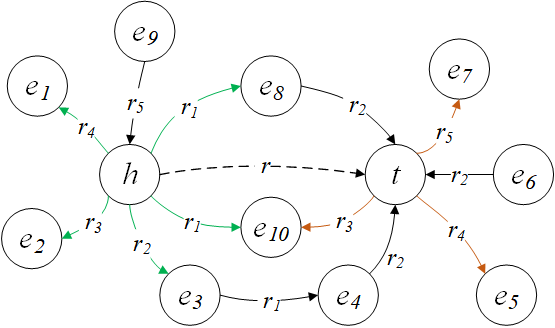
\includegraphics[width=0.45\textwidth]{pic1.png}
  \caption{An illustration of the \emph{triple context} of a triple $(h,r,t)$ in a knowledge graph.}
  \label{pic1}
\end{figure}


\subsection{Path Context}
Path context of a pair of entities is the set of paths that starts from an entity to the other in a KG. It is helpful in modeling the relation and capturing interactions between the pair of entities. Given a pair of entities $(h,t)$, the path context of $(h,t)$ is a set $C_P(h,t)=\{p_i | \forall r_{m_1}, \cdots, r_{m_i}, e_1, \cdots, e_{m_i-1},$ $p_i=(r_{m_1}, \cdots, r_{m_i}), (h,r_{m_1},e_1)\in\mathcal{K}, \cdots, (e_{m_i-1}, r_{m_i}, t)\in\mathcal{K}\}$, where $p_i=$ is a list of relations (labeled edges) through which it can traverse from $h$ to $t$, $m_i$ is the length of path $p_i$. In Figure~\ref{pic1}, the path context between $h$ and $t$ is $C_P(h,t) = \{(r_1, r_2), (r_2, r_1, r_2)\}$. We use the path context to predict the tail entity of a triple given the head entity.

\section{Knowledge Graph Embedding With Attentional Triple Context} \label{sec:pro}


\section{Experiments}\label{sec:set}

\begin{table*} %\small
  \centering
  \caption{Results on FB15k by relation category}
  \label{FB15k_results_by_relation_category}
  \begin{tabular}{c|cccc|cccc}
    \hline
    Task               & \multicolumn{4}{c|}{Predicting head(\textsc{Hits}@10(\%))} & \multicolumn{4}{c}{Predicting tail(\textsc{Hits}@10(\%))} \\
    \hline
    Relation Category  & 1-To-1        & 1-To-N        & N-To-1        & N-To-N        & 1-To-1        & 1-To-N        & N-To-1        & N-To-N \\
    \hline
%    SE                 & 35.6          & 62.6          & 17.2          & 37.5          & 34.9          & 14.6          & 68.3          & 41.3   \\
%    SME(linear)        & 35.1          & 53.7          & 19.0          & 40.3          & 32.7          & 14.9          & 61.6          & 43.3   \\
%    SME(bilinear)      & 30.9          & 69.6          & 19.9          & 38.6          & 28.2          & 13.1          & 76.0          & 41.8   \\
    TransE             & 43.7          & 65.7          & 18.2          & 47.2          & 43.7          & 19.7          & 66.7          & 50.0   \\
    TransH (unif)      & 66.7          & 81.7          & 30.2          & 57.4          & 63.7          & 30.1          & 83.2          & 60.8   \\
    TransH (bern)      & 66.8          & 87.6          & 28.7          & 64.5          & 65.5          & 39.8          & 83.3          & 67.2   \\
    TransR (unif)      & 76.9          & 77.9          & 38.1          & 66.9          & 76.2          & 38.4          & 76.2          & 69.1   \\
    TransR (bern)      & 78.8          & \textbf{89.2} & 34.1          & 69.2          & 79.2          & 37.4          & \textbf{90.4} & 72.1   \\
    CTransR (unif)     & 78.6          & 77.8          & 36.4          & 68.0          & 77.4          & 37.8          & 78.0          & 70.3   \\
    CTransR (bern)     & \textbf{81.5} & 89.0          & 34.7          & 71.2          & \textbf{80.8} & 38.6          & 90.1          & 73.8   \\
    \hline
    ATCE                & 71.0          & 60.3          & \textbf{83.9} & \textbf{81.9} & 70.3          & \textbf{89.9} & 76.0          & \textbf{89.2}   \\
    \hline
\end{tabular}
\end{table*}

\begin{table*} %\small
  \centering
  \caption{Results on FB15k-237 by relation category}
  \label{FB15k-237_results_by_relation_category}
  \begin{tabular}{c|cccc|cccc}
    \hline
    Task               & \multicolumn{4}{c|}{Predicting head(\textsc{Hits}@10(\%))} & \multicolumn{4}{c}{Predicting tail(\textsc{Hits}@10(\%))} \\
    \hline
    Relation Category  & 1-To-1        & 1-To-N        & N-To-1        & N-To-N        & 1-To-1        & 1-To-N        & N-To-1        & N-To-N \\
    \hline
%    SE                 & 35.6          & 62.6          & 17.2          & 37.5          & 34.9          & 14.6          & 68.3          & 41.3   \\
%    SME(linear)        & 35.1          & 53.7          & 19.0          & 40.3          & 32.7          & 14.9          & 61.6          & 43.3   \\
%    SME(bilinear)      & 30.9          & 69.6          & 19.9          & 38.6          & 28.2          & 13.1          & 76.0          & 41.8   \\
    TransE             & 43.7          & 65.7          & 18.2          & 47.2          & 43.7          & 19.7          & 66.7          & 50.0   \\
    TransH (unif)      & 66.7          & 81.7          & 30.2          & 57.4          & 63.7          & 30.1          & 83.2          & 60.8   \\
    TransH (bern)      & 66.8          & 87.6          & 28.7          & 64.5          & 65.5          & 39.8          & 83.3          & 67.2   \\
    TransR (unif)      & 76.9          & 77.9          & 38.1          & 66.9          & 76.2          & 38.4          & 76.2          & 69.1   \\
    TransR (bern)      & 78.8          & \textbf{89.2} & 34.1          & 69.2          & 79.2          & 37.4          & \textbf{90.4} & 72.1   \\
    CTransR (unif)     & 78.6          & 77.8          & 36.4          & 68.0          & 77.4          & 37.8          & 78.0          & 70.3   \\
    CTransR (bern)     & \textbf{81.5} & 89.0          & 34.7          & 71.2          & \textbf{80.8} & 38.6          & 90.1          & 73.8   \\
    \hline
    ATCE                & 71.0          & 60.3          & \textbf{83.9} & \textbf{81.9} & 70.3          & \textbf{89.9} & 76.0          & \textbf{89.2}   \\
    \hline
\end{tabular}
\end{table*}
\subsection{Experimental Setup}

\textbf{\indent Data Set.}
We use two widely-used benchmark data sets FB15k~\cite{BordesUGWY13} and FB15k-237 for evaluation, which are extracted from Freebase. FB15k has\fnum{592213} triples with\fnum{14951} entities and\fnum{1345} relationships.Triples in FB15k-237 are a subset of the FB15K set. FB15k-237 excludes redundant relations and direct training links for held-out triples, with the goal of making the task more realistic ~\cite{Toutanova15}.The two datasets are further divided into three parts for model training, tuning and evaluation. Specifically, we use FB15k and FB15k-237 since their triples are rich and closer to the real popular knowledge graph.

\textbf{Evaluation protocol.}
Following the same protocol used in \cite{BordesUGWY13}, we use \textit{Mean Rank} and \textit{Hits@10} as evaluation protocals of our model. For each test triple $(h,r,t)$, we replace tail head $t$(or the head $h$) with each entity $e$ in $\mathcal{E}$ to generate \emph{corrupted triples} and calculate the scores of each triple using the score function. After ranking the scores in descending order, we then get the rank of the correct entity. \textit{Mean Rank} is the mean of all the predicted ranks, and \textit{Hits@10} denotes the proportion of correct entities ranked in the top 10. Note that, a corrupted triple ranking above a test triple could be valid, which should not be counted as an error. To eliminate the effects of such condition, corrupted triples that already exist in the KG are filtered before ranking. In this case, the setting of evaluation is called "Filter", while the original one is called "Raw". Since this effect ,the "Filter" setting is more preferred. In both settings, a higher Hits@10 imply the better performance of a model.

\textbf{Baselines.}
We use a few outstanding models in recent years as baselines and compare our model with them, including TransE~\cite{BordesUGWY13}, TransH~\cite{WangZFC14}, TransR~\cite{LinLSLZ15} , CTransR~\cite{LinLSLZ15}, PTransE~\cite{LinLLSRL15} and GAKE~\cite{FengHYZ16}. For each baseline model, we first learn representations of all entities and relations. After that the conditional probability of a triple is calculated by the score function, While in ATCE, we construct the triple context with each triple. At last, if the conditional probability of $<h,r,t>$ is larger than $p_r$,  $<h,r,t>$ is regard as a correct triple.

\begin{table} %\small
  \caption{Link prediction results}
  \label{table_link_prediction_results}
  \begin{tabular}{c|cc|cc}
    \hline
    \multirow{2}{*}{Metric}  & \multicolumn{2}{c|}{Mean Rank} & \multicolumn{2}{c}{\textsc{Hits}@10(\%)} \\
                             & Raw          & Filter          & Raw           & Filter          \\
    \hline
%    RESCAL                   & 828          & 683             & 28.4          & 44.1            \\
%    SE                       & 273          & 162             & 28.8          & 39.8            \\
%    SME(linear)              & 274          & 154             & 30.7          & 40.8            \\
%    SME(bilinear)            & 284          & 158             & 31.3          & 41.3            \\
%    LFM                      & 283          & 164             & 26.0          & 33.1            \\
    TransE                   & 243          & 125             & 34.9          & 47.1            \\
    TransH (unif)            & 211          & 84              & 42.5          & 58.5            \\
    TransH (bern)            & 212          & 87              & 45.7          & 64.4            \\
    TransR (unif)            & 226          & 78              & 43.8          & 65.5            \\
    TransR (bern)            & 198          & 77              & 48.2          & 68.7            \\
    CTransR (unif)           & 233          & 82              & 44.0          & 66.3            \\
    CTransR (bern)           & 199          & 75              & 48.4          & 70.2            \\
    PTransE                  & 207          & 58              & 51.4          & \textbf{84.6}   \\
    GAKE                     & 228          & 119             & 44.5          & 64.8            \\
    \hline
    TCE                      & \textbf{110} & \textbf{25}     & \textbf{55.3} & 83.1            \\
    \hline
  \end{tabular}
\end{table}

\textbf{Implementation.}
We construct the knowledge graph using Apache TinkerPop\footnote{\url{http://tinkerpop.apache.org/}}, an open source graph computing framework. In a few cases, the reverse relation, an edge labeled $r^{-1}$ from $t$ to $h$ for the triple $(h,r,t)$, would be useful when representing some patterns in the graph. For instance, the relation path $a \xrightarrow{motherOf} b \xleftarrow{fatherOf} c$, i.e., $(a, motherOf, b)$ and $(c, fatherOf, b)$, indicates a potential relation $marriedTo$ between $a$ and $c$. Therefore, we add reverse relation of each relation into KG. Specifically, for each edge labeled $r$ from $h$ to $t$ in the graph, we add another edge labeled $r^{-1}$ from $t$ to $h$.

For neighbor context generation, it's expensive to consider all the neighbors of each entity in the graph for the reason that there are some entities connecting with a large amount of other entities, which would lead to a huge size of neighbor context. We use sampling to reduce the size of neighbor context. For those entity whose neighbor context size is larger than a fixed size $n$, we sample $n$ neighbors randomly from it's neighbor context. Similarly, a large number of paths between a pair of entities would result in high computational complexity. To solve the problem, firstly, we limit the length of paths by 2-step and 3-step, then, we use random walk to sample $m$ paths between a pair of entities. In our experiment, $n$ and $m$ are all set as 10. Note that for some pairs of entities, there may be no 2 or 3 step relation paths. In such case, we suppose that the relatedness between those pairs of entities are relatively low and the values of $g_P(\cdot, \cdot)$ in Eq.~\eqref{gp} are set as -100. We store all triple contexts in Mongodb\footnote{\url{www.mongodb.org/}},a NoSQL database, that can help us for rapid seeking the context of a specified entity.


We use mini-batch SGD to train our model. We choose the learning rate $\alpha$ of SGD among $\{0.1, 0.01, 0.001\}$, the dimension of embeddings $k$ among $\{50, 75, 100\}$, the batch size $B$ among $\{120, 480,$ $ 960, 1920, 4800\}$. The best parameters are determined by the performance on valid set. The optimal parameters are $\alpha=0.001$, $k=50$ and $B=4800$.

\subsection{Link Prediction}
Link prediction~\cite{BordesUGWY13} is a task to predict the missing head or tail entity in a given triple based on training triples. Metrics \textit{Mean Rank} and \textit{Hits@10} are used to measure the performance of our model.


We collected the result of link prediction in Table~\ref{table_link_prediction_results}. From the results we can see that, our model outperforms other baselines on most of the metrics significantly and consistently, while slightly worse than PTransE on \textsc{Hits}@10. The result implies that triple contexts do improve the performance on link prediction. Although using similar types of contexts in the graph, GAKE's performance is inferior to our model, which shows the superiority of our framework. Note that the experimental results of \textsc{HolE} are absent here, for it uses a different metric, MRR (Mean Reciprocal rank), instead of \textit{Mean rank} for evaluation. But according to \textit{Hits@10} reported in~\cite{NickelRP16}, the results of our model are better than \textsc{HolE}.


In Table~\ref{FB15k_results_by_relation_category} and Table~\ref{FB15k-237_results_by_relation_category}, we show separate evaluation results by category of relationships on FB15k. We can see that ATCE brings promising improvements on modeling complex relations, such as predicting tail of 1-To-N relations, predicting head of N-To-1 relations and N-To-N relations. Specifically, ATCE behaves well when predicting the "N" side of 1-To-N and N-To-1 relations, indicating that valid triples have higher scores than invalid triples in general. In some other simpler scenarios, such as 1-To-1 relations and predicting the "1" side of 1-To-N and N-To-1 relations, the performance of ATCE is still acceptable although not so good as some other baselines, such as TransH and TransR. The results suggest that the incorporation of triple context is helpful when handling complex relations, at the cost of precision in modeling simple relations, which seems complementary to some other baselines.
\subsection{Triple Classification}
We also test our model on triple classification. In this task,given a knowledge base and a triple $<h,r,t>$ we aim to determine whether it is correct or not. FB15K has only positive examples, thus we generated negative triples for FB15K by following strategy of ~\cite{socher2013}. As the result, the classification accuracies on FB15K and FB15k-237 can be compare directly with previous studies. In this task, we choose TransE,TransH,TransR,TransD,NTN and GAKE as baseline models. The parameter values for training TransE,TransH,TransR,TransD,NTN and GAKE are borrowed from their reports.

\begin{table}
 \centering
 \caption{Triple Classification results}
  \label{Triple Classification_results}
\begin{tabular}{c|c|c}
  \hline
  Start & FB15k  & FB15k-237 \\
  \hline
  TransE & 0.81 & 0.82 \\
  TransH & 0.81 & 0.81 \\
  TransR & 0.82 & 0.82 \\
  TransD & 0.87 & 0.87 \\
  GAKE & 0.89 & 0.88 \\
  NTN & 0.41 & 0.42 \\
  \hline
  ATCR & \textbf{0.91} & \textbf{0.92} \\
  \hline
\end{tabular}
\end{table}
In Table ~\ref{Triple Classification_results}, we shows the accuracies of triple classification on two datasets. The context preserving embeddings in general outperform their base model. As the table shows, ATCE always has higher accuracy than TransE,TransH,TransR,TransD,NTN and GAKE. One thing to note is that the improvements by the context preserving embeddings are always observed in FB15k, while those in FB15-237 are small or slightly negative. This can be explained with number of triples with a transitive or symmetric relation in the dataset. In FB15k-237, this kinds of triples are removed from FB15k. Thus the improvement in FB15K is remarkable, our approach outperforms others by 11.04\% in terms of accuracy on average as the triple context brings more information especially relations between entities when learning the knowledge graph representations.

Furthermore, to better understand the attention mechanism in our approach, The examples of path are selected by attention mechanism in path context are shown in Table ~\ref{Attention Results in Path Context}. The number in front each line is the weight score, which is computed by the attention mechanism for each relation. From the examples we can see that ATCE successfully combines structure learning and parameter learning. It not only choose multiple connective path between two entities to capture the complex structure in the knowledge base, but also learn weight score of the path for a specific relation.

\begin{table}
 \centering
 \caption{Attention Results in Path Context}
  \label{Attention Results in Path Context}
  \small
  \setlength{\tabcolsep}{1mm}{
\begin{tabular}{c|l|l}
  \hline
  Weight & Path  & Relation \\
  \hline
  0.45 &  $contains \xrightarrow{} contains $ & $partially\_contains$ \\
  0.35 & $contains \xrightarrow{} nationality$ & $marriage\_location$ \\
  0.24 & $nationality$ & $marriage\_location$ \\
  0.35 & $contains \xrightarrow{} place\_lived$ & $marriage\_location$ \\
  0.2 & $nominated\_for$ & $film\_edited\_by$\\
  0.3 & $nominated \xrightarrow{} award\_nominee$ & $film\_edited\_by$\\
  \hline
\end{tabular}}
\end{table}

For neighbor context, we also use attention mechanism to choose which neighbor is more related for the head. we demonstrate attentions of the 6 different neighbors when they are regards as the neighbor context of the entity $Terminate2:JudgementDay$, which indicates a movie in 1991. Figure ~\ref{pic2}  shows the results, from the results we see two entities, $Action$ and $Sequel$ ,have largest attention to represent the target entity $Terminate2:JudgementDay$, as $Action$  reflects the type of movie while only some of movies have sequels.
\begin{figure}
  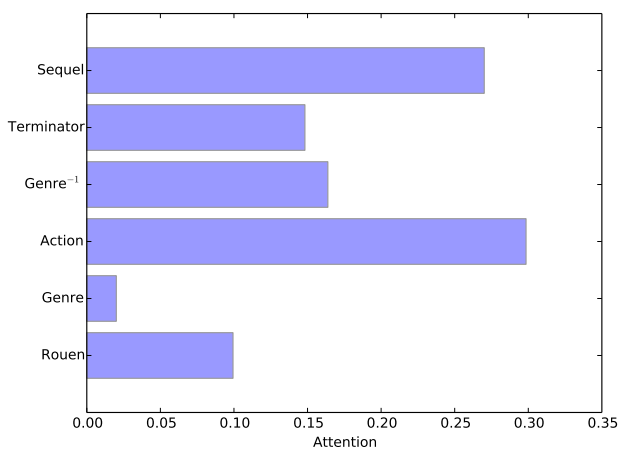
\includegraphics[width=0.45\textwidth]{pic2.png}
  \caption{Attentions for neighbor context of  \emph{Terminate2:JudgementDay}}
  \label{pic2}
\end{figure}









\section{Related Work}\label{sec:rel}



\section{Conclusion}\label{sec:con}
In this paper, we proposed a novel approach to learning disjointness and subclass axioms from incomplete semantic data under OWA. We first applied the type inference algorithm to generate new probabilistic type assertions. We then introduced novel definitions of support and confidence using negative examples as constraints. The experimental results were provided to compare our system with existing one and showed that SIFS-P performs better with respect to precision and recall in most cases.

In the future, we plan to extend the SIFS-P to learn more kinds of axioms such as the axioms with existential restriction, universal restriction and the limited extensional quantification. 



%% The file named.bst is a bibliography style file for BibTeX 0.99c
\bibliographystyle{named}
%\bibliographystyle{unsrt}
\bibliography{bibOfTex}

\end{document}

